
%% bare_jrnl.tex
%% V1.3
%% 2007/01/11
%% by Michael Shell
%% see http://www.michaelshell.org/
%% for current contact information.
%%
%% This is a skeleton file demonstrating the use of IEEEtran.cls
%% (requires IEEEtran.cls version 1.7 or later) with an IEEE journal paper.
%%
%% Support sites:
%% http://www.michaelshell.org/tex/ieeetran/
%% http://www.ctan.org/tex-archive/macros/latex/contrib/IEEEtran/
%% and
%% http://www.ieee.org/



% *** Authors should verify (and, if needed, correct) their LaTeX system  ***
% *** with the testflow diagnostic prior to trusting their LaTeX platform ***
% *** with production work. IEEE's font choices can trigger bugs that do  ***
% *** not appear when using other class files.                            ***
% The testflow support page is at:
% http://www.michaelshell.org/tex/testflow/


%%*************************************************************************
%% Legal Notice:
%% This code is offered as-is without any warranty either expressed or
%% implied; without even the implied warranty of MERCHANTABILITY or
%% FITNESS FOR A PARTICULAR PURPOSE! 
%% User assumes all risk.
%% In no event shall IEEE or any contributor to this code be liable for
%% any damages or losses, including, but not limited to, incidental,
%% consequential, or any other damages, resulting from the use or misuse
%% of any information contained here.
%%
%% All comments are the opinions of their respective authors and are not
%% necessarily endorsed by the IEEE.
%%
%% This work is distributed under the LaTeX Project Public License (LPPL)
%% ( http://www.latex-project.org/ ) version 1.3, and may be freely used,
%% distributed and modified. A copy of the LPPL, version 1.3, is included
%% in the base LaTeX documentation of all distributions of LaTeX released
%% 2003/12/01 or later.
%% Retain all contribution notices and credits.
%% ** Modified files should be clearly indicated as such, including  **
%% ** renaming them and changing author support contact information. **
%%
%% File list of work: IEEEtran.cls, IEEEtran_HOWTO.pdf, bare_adv.tex,
%%                    bare_conf.tex, bare_jrnl.tex, bare_jrnl_compsoc.tex
%%*************************************************************************

% Note that the a4paper option is mainly intended so that authors in
% countries using A4 can easily print to A4 and see how their papers will
% look in print - the typesetting of the document will not typically be
% affected with changes in paper size (but the bottom and side margins will).
% Use the testflow package mentioned above to verify correct handling of
% both paper sizes by the user's LaTeX system.
%
% Also note that the "draftcls" or "draftclsnofoot", not "draft", option
% should be used if it is desired that the figures are to be displayed in
% draft mode.
%
\documentclass[journal]{IEEEtran}

\usepackage{blindtext}
\usepackage{graphicx}
\usepackage{biblatex}
\usepackage{float}
\graphicspath{ {images/} }
% Some very useful LaTeX packages include:
% (uncomment the ones you want to load)


% *** MISC UTILITY PACKAGES ***
%
%\usepackage{ifpdf}
% Heiko Oberdiek's ifpdf.sty is very useful if you need conditional
% compilation based on whether the output is pdf or dvi.
% usage:
% \ifpdf
%   % pdf code
% \else
%   % dvi code
% \fi
% The latest version of ifpdf.sty can be obtained from:
% http://www.ctan.org/tex-archive/macros/latex/contrib/oberdiek/
% Also, note that IEEEtran.cls V1.7 and later provides a builtin
% \ifCLASSINFOpdf conditional that works the same way.
% When switching from latex to pdflatex and vice-versa, the compiler may
% have to be run twice to clear warning/error messages.






% *** CITATION PACKAGES ***
%
%\usepackage{cite}
% cite.sty was written by Donald Arseneau
% V1.6 and later of IEEEtran pre-defines the format of the cite.sty package
% \cite{} output to follow that of IEEE. Loading the cite package will
% result in citation numbers being automatically sorted and properly
% "compressed/ranged". e.g., [1], [9], [2], [7], [5], [6] without using
% cite.sty will become [1], [2], [5]--[7], [9] using cite.sty. cite.sty's
% \cite will automatically add leading space, if needed. Use cite.sty's
% noadjust option (cite.sty V3.8 and later) if you want to turn this off.
% cite.sty is already installed on most LaTeX systems. Be sure and use
% version 4.0 (2003-05-27) and later if using hyperref.sty. cite.sty does
% not currently provide for hyperlinked citations.
% The latest version can be obtained at:
% http://www.ctan.org/tex-archive/macros/latex/contrib/cite/
% The documentation is contained in the cite.sty file itself.






% *** GRAPHICS RELATED PACKAGES ***
%
\ifCLASSINFOpdf
  % \usepackage[pdftex]{graphicx}
  % declare the path(s) where your graphic files are
  % \graphicspath{{../pdf/}{../jpeg/}}
  % and their extensions so you won't have to specify these with
  % every instance of \includegraphics
  % \DeclareGraphicsExtensions{.pdf,.jpeg,.png}
\else
  % or other class option (dvipsone, dvipdf, if not using dvips). graphicx
  % will default to the driver specified in the system graphics.cfg if no
  % driver is specified.
  % \usepackage[dvips]{graphicx}
  % declare the path(s) where your graphic files are
  % \graphicspath{{../eps/}}
  % and their extensions so you won't have to specify these with
  % every instance of \includegraphics
  % \DeclareGraphicsExtensions{.eps}
\fi
% graphicx was written by David Carlisle and Sebastian Rahtz. It is
% required if you want graphics, photos, etc. graphicx.sty is already
% installed on most LaTeX systems. The latest version and documentation can
% be obtained at: 
% http://www.ctan.org/tex-archive/macros/latex/required/graphics/
% Another good source of documentation is "Using Imported Graphics in
% LaTeX2e" by Keith Reckdahl which can be found as epslatex.ps or
% epslatex.pdf at: http://www.ctan.org/tex-archive/info/
%
% latex, and pdflatex in dvi mode, support graphics in encapsulated
% postscript (.eps) format. pdflatex in pdf mode supports graphics
% in .pdf, .jpeg, .png and .mps (metapost) formats. Users should ensure
% that all non-photo figures use a vector format (.eps, .pdf, .mps) and
% not a bitmapped formats (.jpeg, .png). IEEE frowns on bitmapped formats
% which can result in "jaggedy"/blurry rendering of lines and letters as
% well as large increases in file sizes.
%
% You can find documentation about the pdfTeX application at:
% http://www.tug.org/applications/pdftex





% *** MATH PACKAGES ***
%
%\usepackage[cmex10]{amsmath}
% A popular package from the American Mathematical Society that provides
% many useful and powerful commands for dealing with mathematics. If using
% it, be sure to load this package with the cmex10 option to ensure that
% only type 1 fonts will utilized at all point sizes. Without this option,
% it is possible that some math symbols, particularly those within
% footnotes, will be rendered in bitmap form which will result in a
% document that can not be IEEE Xplore compliant!
%
% Also, note that the amsmath package sets \interdisplaylinepenalty to 10000
% thus preventing page breaks from occurring within multiline equations. Use:
%\interdisplaylinepenalty=2500
% after loading amsmath to restore such page breaks as IEEEtran.cls normally
% does. amsmath.sty is already installed on most LaTeX systems. The latest
% version and documentation can be obtained at:
% http://www.ctan.org/tex-archive/macros/latex/required/amslatex/math/





% *** SPECIALIZED LIST PACKAGES ***
%
%\usepackage{algorithmic}
% algorithmic.sty was written by Peter Williams and Rogerio Brito.
% This package provides an algorithmic environment fo describing algorithms.
% You can use the algorithmic environment in-text or within a figure
% environment to provide for a floating algorithm. Do NOT use the algorithm
% floating environment provided by algorithm.sty (by the same authors) or
% algorithm2e.sty (by Christophe Fiorio) as IEEE does not use dedicated
% algorithm float types and packages that provide these will not provide
% correct IEEE style captions. The latest version and documentation of
% algorithmic.sty can be obtained at:
% http://www.ctan.org/tex-archive/macros/latex/contrib/algorithms/
% There is also a support site at:
% http://algorithms.berlios.de/index.html
% Also of interest may be the (relatively newer and more customizable)
% algorithmicx.sty package by Szasz Janos:
% http://www.ctan.org/tex-archive/macros/latex/contrib/algorithmicx/




% *** ALIGNMENT PACKAGES ***
%
%\usepackage{array}
% Frank Mittelbach's and David Carlisle's array.sty patches and improves
% the standard LaTeX2e array and tabular environments to provide better
% appearance and additional user controls. As the default LaTeX2e table
% generation code is lacking to the point of almost being broken with
% respect to the quality of the end results, all users are strongly
% advised to use an enhanced (at the very least that provided by array.sty)
% set of table tools. array.sty is already installed on most systems. The
% latest version and documentation can be obtained at:
% http://www.ctan.org/tex-archive/macros/latex/required/tools/


%\usepackage{mdwmath}
%\usepackage{mdwtab}
% Also highly recommended is Mark Wooding's extremely powerful MDW tools,
% especially mdwmath.sty and mdwtab.sty which are used to format equations
% and tables, respectively. The MDWtools set is already installed on most
% LaTeX systems. The lastest version and documentation is available at:
% http://www.ctan.org/tex-archive/macros/latex/contrib/mdwtools/


% IEEEtran contains the IEEEeqnarray family of commands that can be used to
% generate multiline equations as well as matrices, tables, etc., of high
% quality.


%\usepackage{eqparbox}
% Also of notable interest is Scott Pakin's eqparbox package for creating
% (automatically sized) equal width boxes - aka "natural width parboxes".
% Available at:
% http://www.ctan.org/tex-archive/macros/latex/contrib/eqparbox/





% *** SUBFIGURE PACKAGES ***
%\usepackage[tight,footnotesize]{subfigure}
% subfigure.sty was written by Steven Douglas Cochran. This package makes it
% easy to put subfigures in your figures. e.g., "Figure 1a and 1b". For IEEE
% work, it is a good idea to load it with the tight package option to reduce
% the amount of white space around the subfigures. subfigure.sty is already
% installed on most LaTeX systems. The latest version and documentation can
% be obtained at:
% http://www.ctan.org/tex-archive/obsolete/macros/latex/contrib/subfigure/
% subfigure.sty has been superceeded by subfig.sty.



\hyphenation{op-tical net-works semi-conduc-tor}


\begin{document}
\title{Measuring the engagement of a museum visitor in interactive museum exhibits}
%

\author{Francisco~Arce,
        Mario~Garcia-Valdez
        % <-this % stops a space
\thanks{Pending}% <-this % stops a space
}

% note the % following the last \IEEEmembership and also \thanks - 
% these prevent an unwanted space from occurring between the last author name
% and the end of the author line. i.e., if you had this:
% 
% \author{....lastname \thanks{...} \thanks{...} }
%                     ^------------^------------^----Do not want these spaces!
%
% a space would be appended to the last name and could cause every name on that
% line to be shifted left slightly. This is one of those "LaTeX things". For
% instance, "\textbf{A} \textbf{B}" will typeset as "A B" not "AB". To get
% "AB" then you have to do: "\textbf{A}\textbf{B}"
% \thanks is no different in this regard, so shield the last } of each \thanks
% that ends a line with a % and do not let a space in before the next \thanks.
% Spaces after \IEEEmembership other than the last one are OK (and needed) as
% you are supposed to have spaces between the names. For what it is worth,
% this is a minor point as most people would not even notice if the said evil
% space somehow managed to creep in.



% The paper headers
\markboth{Journal of Class Files,~Vol.~6, No.~1, February~2016}%
{Shell \MakeLowercase{\textit{et al.}}: Bare Demo of IEEEtran.cls for Journals}
% The only time the second header will appear is for the odd numbered pages
% after the title page when using the twoside option.
% 
% *** Note that you probably will NOT want to include the author's ***
% *** name in the headers of peer review papers.                   ***
% You can use \ifCLASSOPTIONpeerreview for conditional compilation here if
% you desire.




% If you want to put a publisher's ID mark on the page you can do it like
% this:
%\IEEEpubid{0000--0000/00\$00.00~\copyright~2007 IEEE}
% Remember, if you use this you must call \IEEEpubidadjcol in the second
% column for its text to clear the IEEEpubid mark.



% use for special paper notices
%\IEEEspecialpapernotice{(Invited Paper)}




% make the title area
\maketitle


\begin{abstract}
\boldmath
Modern interactive museums offer visitors a dynamic learning environment, promoting exploration and encourage the excitement of discovery as visitors learn new concepts, as they are free to interact with the exhibits. In this paper we propose an architecture for an interactive learning environment (ILE) using a collection of commodity devices: a set of displays where different content is presented, a set of mobile devices for each visitor to interact and a Kinect sensor. The engagement affective state is predicted using various classifiers and a database of readings from the Kinect sensor. The architecture also addresses the problem of content distribution among devices.  A case study of an interactive exhibit held in classrooms. The participants were students of Technologic Institute of Tijuana. Experimental results show that the proposed approach can predict the engagement affective state.

\end{abstract}
% IEEEtran.cls defaults to using nonbold math in the Abstract.
% This preserves the distinction between vectors and scalars. However,
% if the journal you are submitting to favors bold math in the abstract,
% then you can use LaTeX's standard command \boldmath at the very start
% of the abstract to achieve this. Many IEEE journals frown on math
% in the abstract anyway.

% Note that keywords are not normally used for peerreview papers.
\begin{IEEEkeywords}
Interactive, Environment, Kinect 2.0, Affective.
\end{IEEEkeywords}






% For peer review papers, you can put extra information on the cover
% page as needed:
% \ifCLASSOPTIONpeerreview
% \begin{center} \bfseries EDICS Category: 3-BBND \end{center}
% \fi
%
% For peerreview papers, this IEEEtran command inserts a page break and
% creates the second title. It will be ignored for other modes.
\IEEEpeerreviewmaketitle



\section{Introduction}


A museum is a public or private institution at the service of the society and its development. These exhibit sets of objects and information that reflect some aspect of human existence or its environment. The museum dates back to the Greco-Roman period, since museums have undergone many changes in terms of how to present the information thanks to technological advances that have emerged, this change has been most noticeable in the last century to date.

In addition to technology there are new techniques and methods to improve the user experience in these museums as interaction, user preferences, virtual and mixed realities among others. Since its beginnings the main objective of museums has been to preserve the cultural heritage, but also make information shown attractive to public in general, this part is a big challenge because each person thinks and assimilates information differently and one of the ways to solve this problem is by making the content adaptive.
Interactive museums have been multiplying in recent year, many of which the idea of attracting the public using new technologies, currently there are studies that seek ways to solve the problem of making more attractive exhibits for the museum visitors as it does (aoki 2002; aoki 2002) where their electronic guidebook allows users to share auditory information (They hear each other) using a technologically mediated audio eavesdropping mechanism.

Reilly 2007 uses another approach oriented towards audio-visual experience where literary information shows through high large screens where the user can interact with the museum with touch screens.Others besides dealing with how to present information have involved more with the user from using their personal information to use methods to predict the state of mind. In affective computing there are several affective states but one that goes hand in hand with learning which is the engagement, like all state of mind is difficult to identify.Allen tell us how to design exhibits and how not make it anti-engagement like using lots of content in multiple displays.   
In this paper we propose the architecture of an interactive environment which consists of the distribution of multimedia content in an exhibit where the content is displayed in sets of learning objects which we call environmental learning object, a simple sequenced implementation which will make the task of a museum guide establishing the order of the learning activities. And finally we use the second-generation Kinect sensor to capture video of the user and predict an emotion based on this catalog the exhibition state as something that engages the user or something that does not engage the user. To test this architecture we conducted an experiment in an interactive museum where we generate a learning activity, at the end of the activity we surveyed the user to obtain information from the user experience and affective state and compare it against the pronostic of the affective state and identify the least interesting activities.


\section {Background}

\subsection {Interactive museums}
Museums at the present are exploring new digital and mobile technologies to enhance the visitor experience. Initiatives go beyond technology within exhibits, but also include more widespread use of technology to create interactive experiences for visitors throughout a museum and remote experiences for those who can not get there.
\subsection {Intelligent Learning Environments}
Intelligent Learning Environments (ILE) are based in learning environments where students and teachers can create knowledge. In other words, the environment represents a cognitive space for a learning community. The ILE seeks to provide adaptive navigation and adaptive sequencing as is commented on  \cite{rondon89}, [10] and [15].The adaptive navigation presents the content of a course in optimized order, where the optimization criteria takes into consideration the learner's backgrounds and performance, whereas adaptive sequencing is defined as the process for selection of learning objects from a digital repository and sequencing them in a way which is appropriated for the targeted learning community or individuals. 
\subsection {Affective Computing}
Affective computing is the human-computer interaction in which a device has the ability to detect and respond to the emotions of the user and other stimulus properly. A computing device with this capability could gather the signals to the user emotion from a variety of sources. Facial expressions, posture, gestures, speech, strength and pace of keystrokes and temperature changes of hand on a mouse all can mean changes in the emotional state of the user, and these can be detected and interpreted by a computer. A camera is used to capture images of the user and the data is processed algorithms to produce meaningful information. Voice recognition and gesture recognition are some of the other technologies being explored for affective computing applications.



\subsection {Kinect 2.0}

\section {Method}
\setlength{\parskip}{10pt}
%Este estudio esta dividido en 2, en la primera parte se realizo con visitantes del museo el trompo de tijuana donde participaron 21 usuarios divididos en 2 grupos, el primero cuenta con 10 usuarios de entre 6 y 11 años 50\% hombres y 50\% mujeres y el segundo grupo de consistia de 11 usuarios de 11 años en adelante 66\% hombres 44\% mujeres. En la segunda parte del estudio se utilizaron 41 usuarios del instituto tecnologico de tijuana con edades entre los 18 y 50 años 66\% hombres 34\% mujeres.

This study is divided into 2, the first part was conducted with visitors to the museum's spin tijuana where 21 users divided into 2 groups participated, the first has 10 users between 6 and 11 years 50 \% men and 50 \% women and the second group consisted of 11 users 11 and older 66 \% men 44 \% women. In the second part of the study 41 users of the Technological Institute of Tijuana were used aged between 18 and 50 years 66 \% men 34 \% women.

%Para este estudio se requiere mostrar imagenes, videos y de alguna forma observar al usuario, por ello se utilizaron diversos dispositivos que cumplian con estas necesidades como una computadora que hacia de servidor, 2 laptops, 1 tablet de 7 pulgadas, audifonos, 3 proyectores 2 monitores, camaras, sensores (Kinect 2.0) etc.

For this study is required to show images, videos and somehow observe the user, that is why many devices that met these needs as a computer to server, 2 laptops, one 7-inch tablet, headphones, 3 projectors, 2 monitors, cameras, sensors (Kinect 2.0) etc. were used.
    

%En la primer parte del estudio se sumergio a los usuarios en un exhibidor que les proporcionaba informacion visual y auditiva como se observa en la figura 1 sobre un tema que seleccionamos en base a varios criterios, como la localidad de el estudio en esta ocacion era un museo interactivo y se aproximava la festividad de el dia del niño tratamos de utilizar un tema simple y que aportara conciencia por eso decidimos utilizar el tema del agua donde se mostro informacion como los usos de esta misma, su ciclo, las formas de energia que podia generar, la salud, y la importancia de ella para el planeta. A cada uno de los usuarios se les generaba una cuenta en el sistema para poder registrar su actividad, despues de esto se les hacia una breve explicacion de como funcionaba el exhibidor los demas a base de observacion ya no requirieron esta explicacion. El usuario tomaba una tablet que era la forma en que el usuario interactuaba con el exhibidor, con el tenia el control del flujo de la informacion, como la informacion era una secuencia al final la ultima actividad era un questionario sobre la informacion que recibio ademas de una encuesta.
\begin{figure}[H]
	\centering
	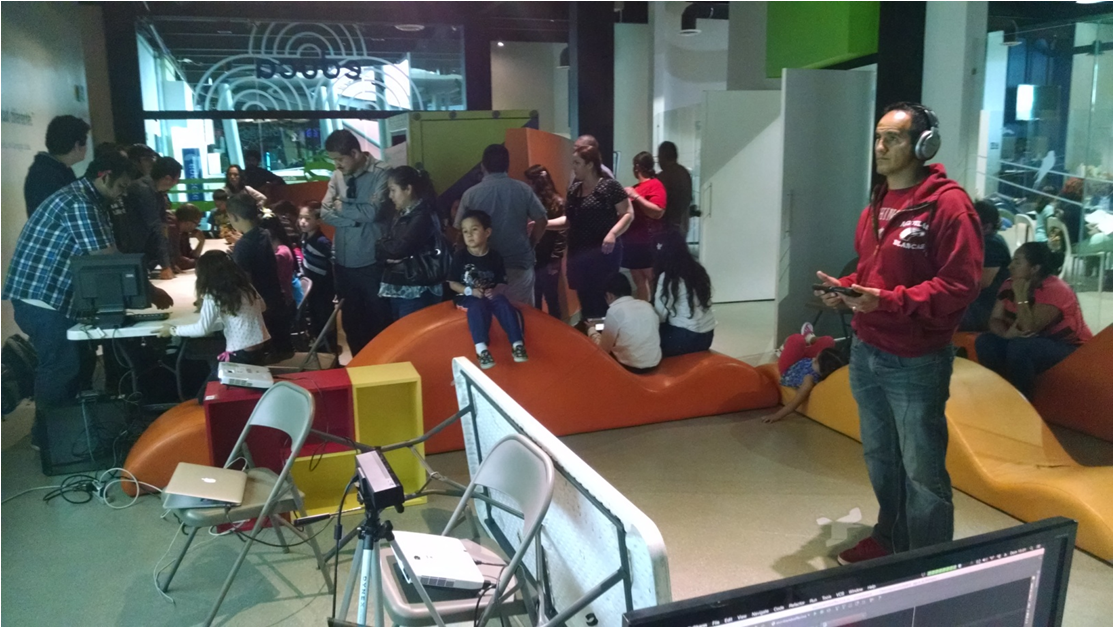
\includegraphics [width=90mm] {tromp.PNG}
	\label{fig:Figure 1}
	Fig 1. User interacting with the environment.
\end{figure}

In the first part of the study users immersed in an exhibitor that gave them visual and aural information as shown in Figure 1 on a topic selected based on various criteria, such as the location of the study on this occasion was a interactive museum and the festival of children's day approaching we try to use a simple theme and it will bring awareness so we decided to use the theme of water where information was displayed as the uses of the same, its cycle, forms of energy that could generate, health, and the importance of it for the planet. Each of users are generating an account on the system to register their activity, after that we were made a brief explanation of how it worked the exhibitor others based on observation no longer required this explanation. The user took a tablet that was the how the user interacted with the exhibitor, with which had control of the flow of information, as the information was a sequence at the end of the last activity was a questionnaire on the information received besides a survey.

%En la segunda parte del estudio fue muy parecido al primero solo que tubo unas pequeñas modificaciones y adiciones figura 3, ahora el usuario ya no tenia control de flujo solo observo y ademas de observar al usuario ahora se le tomo video y se incluyo el sensor, el tema de la exhibicion fueron los video juegos y el cine como las edades de los usarios irian desde casi los 17 años en adelante podrian ser temas de interez. De la misma forma cada que en la primera parte cada usuario contaba con una cuenta para registrar la actividad solo que esta ocacion se registrarian los datos arrojados por el sensor y los videos capturados por la camara, y de la misma forma que en la primera parte al final se encuesto al usuario.  

The second part of the study was very similar to the first one that had some small modifications and additions, now the user no longer had control flow only observe and also to observe the user now will take video and sensor, the theme of the exhibition were video games and film as the age of the users would go for almost 17 years and older could be topics of their interest. In the same way as in the first part each user had an account to record the activity only this occasion the data produced by the sensor and videos captured by the camera would be recorded, and in the same way as in the first part at the end we surveyed the users.
     
\begin{figure}[H]
	\centering
	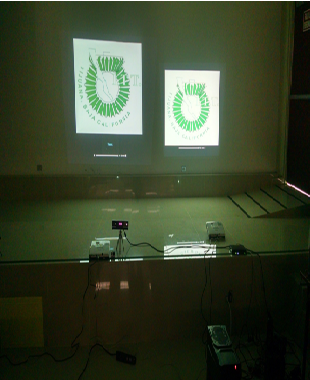
\includegraphics[width=80mm,height=80mm]{frenteexhi.PNG}
	\label{fig:Figure 3}
	Fig 3. Front display.
\end{figure}


%Para la primer parte del estudio se recabaron datos de la encuesta realizada al final, en la segunda como utilizamos datos de sensores los datos eran un poco mas complejos, primero habia que analizar visual/manualmente al usuario donde el observador determinaba si el usuario estaba poniendo atencion a lo que veia o se distraia y con base en eso asignaba un nivel de atencion en una escala de 1 a 3 donde 1 era poca atencion 2 atencion media y 3 muy atento. La otra forma de obtener informacion del usuario que era por kinect es un poco mas compleja ya que el sensor aporta bastante informacion el sensor al detectar a un usuario puede dar:

For the first part of the study we get data from the survey conducted at the end, in the second they are collected and used data from sensors, this data were a bit more complex, first we need an observer to evaluate the user manually, where the observer determined whether the user was putting attention to what he saw or distracted and based on that assigned a level of attention on a scale of 1 to 3 where 1 is little attention 2 average attention and 3 very attentive. The other way to obtain user information was by Kinect Sensor and is a bit more complex because the sensor provides enough information the sensor detects a user can give:

\begin{itemize}
 \item engage
 \item looking away
 \item happy
 \item left eye closed
 \item right eye closed
 \item mouth open
 \item mouth moved 
 \item wearing glasses
 \item yaw pitch and roll of the face
\end{itemize}

%Cada uno de estos datos el sensor asiganaba uno de los siguientes valores Yes, No, Maybe y Unknow; los datos de unknow fueron descartados ya que en la documentacion del sensor decia que este dato podia ser "`no sensado"' y por lo tanto considerado como dato no valido. Solo en la posicion de rostro el resultado era numerico, el sensor generaba un promedio de 14 registros por segundo de estos valores en ocaciones menos cuando por poco tiempo el sensor perdia al usuario pero usualmente era entre 1 y 10 segundos. La actividad completa se realizaba en 4 minutos con 10 segundos por lo que si el sensor no perdio de vista al usuario durante toda la actividad hacia al rededor de 3500 registros. De la lista anterior de datos decidimos utilizar solo engage, happy y looking away los demas aunque estan capturados los descartamos ya que no son relevantes para lo que estamos midiendo. al obtener resultados textuales realizamos una normalizacion haciendo un conteo de cada evento cada 10 segundos ya que los datos generados por el sensor son textuales se normalizaron asignando numeros a los strings por ejemplo Yes = 2, Maybe = 1 y No = 0 entonces por cada 10 segundos de actividad se contabilizaban los Yes, Maybe y No      

Each of these data the sensor assigned one of the following Yes, No, Maybe and Unknown values; unknown data were discarded since in the sensor documentation was saying that this data could be "not sensing" and therefore not considered valid data. Only in the face position was a numerical data, the sensor generated an average of 14 records per second of these values sometimes less for a short time when the sensor lost sight of the user  but was usually between 1 to 10 seconds. 

%[H] sirve para obligar a la figura o la tabla a estar en ese lugar

\begin{figure}[H]
	\centering
	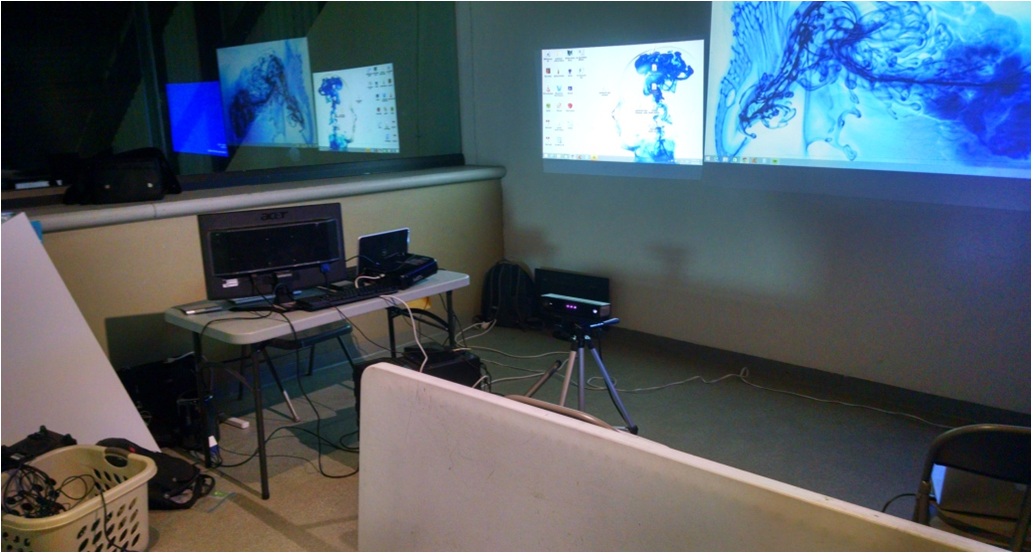
\includegraphics [width=90mm]{tromp2.PNG}
	\label{fig:Figure 2}
	Fig 2. Front view.
\end{figure}

Full activity was carried out in 4 minutes 10 seconds so if the sensor not lose sight of the user throughout the activity It generates about 3500 records. From the above list of data we decided to use only engage, looking away happy and others are captured but used as they are not relevant to what we are measuring. To get textual results perform a normalization by a count of each event every 10 seconds since the data generated by the sensor are textual normalized by assigning numbers to strings for example Yes = 2, Maybe = 1 and No = 0 then for every 10 seconds of activity the Yes, No and Maybe was counted.

%Como la actividad duraba 4:10 decidimos contar los eventos del sensor cada 10 segundos, al final obteniamos un promedio de 140 registros por cada periodo de 10 segundos. Aqui surgio un problema, como la cantidad de registros variaba por usuario tubimos que pensar en como normalizar estos datos, como los registros eran contabilizados y distribuidos en si, tal vez y no la solucion fue sacar el porcentaje de cada uno de los registros obtenidos por lo que de esa manera ya podiamos manejar los datos del sensor.
As the activity lasted 4:10 we decided to count the sensor event every 10 seconds, at the end we gained an average of 140 records for each period of 10 seconds. Here I was a problem, as the number of records varied by user we had to think about how to normalize this data, as records were recorded and distributed yes, maybe, no the solution was to take a percentage of each of the records obtained by which thus we could handle and sensor data.

\section {Results}

%Los resultados al igual que en las otras secciones estan divididos en 2.
The results as in the other sections are divided into two.
%El primer experimento que se llevo a cabo en el museo interactivo donde se utilizaron 2 grupos de usuarios y obtubieron los siguientes resultados, En la tabla 1 se muestra el resultado de las primeras 4 preguntas de la encuesta, en la segunda tabla se muestra las ultimas 4 preguntas hechas. Recordando que fueron 11 los usuarios encuestados.
The first experiment was carried out at the interactive museum where two user groups were used and obtained the following results Table 1 shows the result of the first 4 survey questions in the second table shown the last 4 questions asked. Recalling that there were 11 respondents users.


% la tomamos de 2 encuestas Ya que tubimos los datos organizados y normalizados 

\begin{table}[H]
\caption{: Results of the survey taken by the group 1 in the interactive museum Part 1. }
\begin{tabular}{l*{4}{c}r}
									& Q1 & Q2 & Q3 & Q4  \\
\hline
Standard Deviation & 0.504524979	& 0.687551651	& 0.820199532	& 1.009049958	\\
Mean & 4.636363636	& 4.454545455	& 4.454545455	& 4.272727273	 \\
\hline
\end{tabular}	
\end{table}

\begin{table}[H]
\caption{: Results of the survey taken by the group 2 in the interactive museum Part 2. }
\begin{tabular}{l*{4}{c}r}
									& Q5 & Q6 & Q7 & Q8 \\
\hline
Standard Deviation & 0.820199532	& 0.646669791	& 0.687551651	& 0.646669791 \\
Mean & 4.454545455	& 4.727272727	& 4.454545455	& 4.727272727 \\
\hline
\end{tabular}	
 
\end{table}
 
%En la segunda parte del experimento se encuesto al segundo grupo de usuarios y los resultados se muestran en la tabla 3. 
In the second part of the experiment was the second group of surveyed users and the results are shown in Table 3.

\begin{table}[H]
\caption{: Results of the survey taken by the group 2 in the interactive museum. }
\begin{tabular}{l*{4}{c}r}
									& Q1 & Q2 & Q3 & Q4  \\
\hline
Standard Deviation  & 0.971825316	& 0.483045892	& 0.483045892	& 0.843274043	\\
Mean & 4.5	& 4.7	& 4.7	& 4.4	 \\
\hline
\end{tabular}	
\end{table}


%Los resultados del segundo experimento fueron arrojados por 4 clasificadores el primero de ellos fue 
%The results of the second experiment were cast for 4 classifiers the first was Decision tree with an accuracy: 88.42\% +/- 5.17\% (mikro: 88.44\%) kappa: 0.803 +/- 0.088 (mikro: 0.804) in Table 4 shows the confusion matrix of the results of this classifier.

\begin{table}[H]
\caption{: Results of the prediction on the level of attention of the user using Decision tree. }
\begin{tabular}{l*{4}{c}r}
									& True Low & True Mid & True High & Class Precision \\
\hline
Prediction Low  & 141 & 25 & 2 & 83.93\% \\
Prediction Mid  & 14 & 77 & 16 & 71.96\%  \\
Prediction High & 3 & 11 & 325 & 95.87\%  \\
\hline
Class Recall    & 89.24\% & 68.14\% & 94.75\% &  \\
\end{tabular}	
\end{table}

%el cual tubo en la tabla 4 se puede obserbar la matriz de confusion de lso resultados de este clasificador.
%The next classifier was KNN with an accuracy: 87.77\% +/- 4.13\% (mikro: 87.79\%) kappa: 0.792 +/- 0.069 (mikro: 0.7091) in Table 4 shows the confusion matrix of the results of this classifier.

\begin{table}[H]
\caption{: Results of the prediction on the level of attention of the user using KNN. }
\begin{tabular}{l*{6}{c}r}
									& True Low & True Mid & True High & Class Precision \\
\hline
Prediction Low  & 133 & 19 & 3 & 89.13\% \\
Prediction Mid  & 22 & 78 & 12 & 70.33\%  \\
Prediction High & 3 & 16 & 328 & 84.94\%  \\
\hline
Class Recall    & 84.18\% & 69.03\% & 495.63\% &  \\
\end{tabular}	
\end{table}

%The next classifier was Bayes with an accuracy: 83.69\% +/- 4.57\% (mikro: 83.71\%) kappa: 0.712 +/- 0.079 (mikro: 0.712) in Table 4 shows the confusion matrix of the results of this classifier.

\begin{table}[H]
\caption{: Results of the prediction on the level of attention of the user using Bayes. }
\begin{tabular}{l*{3}{c}r}
									& True Low & True Mid & True High & Class Precision \\
\hline
Prediction Low  & 123 & 13 & 2 & 85.81\% \\
Prediction Mid  & 13 & 88 & 13 & 69.64\%  \\
Prediction High & 22 & 14 & 327 & 94.52\%  \\
\hline
Class Recall    & 84.18\% & 69.03\% & 95.63\% &  \\
\end{tabular}	
\end{table}

%And the last classifier was Neural Networks with an accuracy: 91.03\% +/- 3.68\% (mikro: 88.44\%) in Table 4 shows the confusion matrix of the results of this classifier.


\begin{table}[H]
\caption{: Results of the prediction on the level of attention of the user using NN. }
\begin{tabular}{l*{3}{c}r}
									& True Low & True Mid & True High & Class Precision \\
\hline
Prediction Low  & 144 & 11 & 3 & 85.81\% \\
Prediction Mid  & 12 & 88 & 13 & 69.64\%  \\
Prediction High & 2 & 14 & 327 & 94.52\%  \\
\hline
Class Recall    & 84.18\% & 69.03\% & 95.63\% &  \\
\end{tabular}	
\end{table}

% needed in second column of first page if using \IEEEpubid
%\IEEEpubidadjcol

% An example of a floating figure using the graphicx package.
% Note that \label must occur AFTER (or within) \caption.
% For figures, \caption should occur after the \includegraphics.
% Note that IEEEtran v1.7 and later has special internal code that
% is designed to preserve the operation of \label within \caption
% even when the captionsoff option is in effect. However, because
% of issues like this, it may be the safest practice to put all your
% \label just after \caption rather than within \caption{}.
%
% Reminder: the "draftcls" or "draftclsnofoot", not "draft", class
% option should be used if it is desired that the figures are to be
% displayed while in draft mode.
%
%\begin{figure}[!t]
%\centering
%\includegraphics[width=2.5in]{myfigure}
% where an .eps filename suffix will be assumed under latex, 
% and a .pdf suffix will be assumed for pdflatex; or what has been declared
% via \DeclareGraphicsExtensions.
%\caption{Simulation Results}
%\label{fig_sim}
%\end{figure}

% Note that IEEE typically puts floats only at the top, even when this
% results in a large percentage of a column being occupied by floats.


% An example of a double column floating figure using two subfigures.
% (The subfig.sty package must be loaded for this to work.)
% The subfigure \label commands are set within each subfloat command, the
% \label for the overall figure must come after \caption.
% \hfil must be used as a separator to get equal spacing.
% The subfigure.sty package works much the same way, except \subfigure is
% used instead of \subfloat.
%
%\begin{figure*}[!t]
%\centerline{\subfloat[Case I]\includegraphics[width=2.5in]{subfigcase1}%
%\label{fig_first_case}}
%\hfil
%\subfloat[Case II]{\includegraphics[width=2.5in]{subfigcase2}%
%\label{fig_second_case}}}
%\caption{Simulation results}
%\label{fig_sim}
%\end{figure*}
%
% Note that often IEEE papers with subfigures do not employ subfigure
% captions (using the optional argument to \subfloat), but instead will
% reference/describe all of them (a), (b), etc., within the main caption.


% An example of a floating table. Note that, for IEEE style tables, the 
% \caption command should come BEFORE the table. Table text will default to
% \footnotesize as IEEE normally uses this smaller font for tables.
% The \label must come after \caption as always.
%
%\begin{table}[!t]
%% increase table row spacing, adjust to taste
%\renewcommand{\arraystretch}{1.3}
% if using array.sty, it might be a good idea to tweak the value of
% \extrarowheight as needed to properly center the text within the cells
%\caption{An Example of a Table}
%\label{table_example}
%\centering
%% Some packages, such as MDW tools, offer better commands for making tables
%% than the plain LaTeX2e tabular which is used here.
%\begin{tabular}{|c||c|}
%\hline
%One & Two\\
%\hline
%Three & Four\\
%\hline
%\end{tabular}
%\end{table}


% Note that IEEE does not put floats in the very first column - or typically
% anywhere on the first page for that matter. Also, in-text middle ("here")
% positioning is not used. Most IEEE journals use top floats exclusively.
% Note that, LaTeX2e, unlike IEEE journals, places footnotes above bottom
% floats. This can be corrected via the \fnbelowfloat command of the
% stfloats package.



\section{Conclusion}
Conclusion aqui.





% if have a single appendix:
%\appendix[Proof of the Zonklar Equations]
% or
%\appendix  % for no appendix heading
% do not use \section anymore after \appendix, only \section*
% is possibly needed

% use appendices with more than one appendix
% then use \section to start each appendix
% you must declare a \section before using any
% \subsection or using \label (\appendices by itself
% starts a section numbered zero.)
%


\appendices
\section{Proof of the First Zonklar Equation}
Some text for the appendix.

% use section* for acknowledgement
\section*{Acknowledgment}


The authors would like to thank...


% Can use something like this to put references on a page
% by themselves when using endfloat and the captionsoff option.
\ifCLASSOPTIONcaptionsoff
  \newpage
\fi



% trigger a \newpage just before the given reference
% number - used to balance the columns on the last page
% adjust value as needed - may need to be readjusted if
% the document is modified later
%\IEEEtriggeratref{8}
% The "triggered" command can be changed if desired:
%\IEEEtriggercmd{\enlargethispage{-5in}}

% references section

% can use a bibliography generated by BibTeX as a .bbl file
% BibTeX documentation can be easily obtained at:
% http://www.ctan.org/tex-archive/biblio/bibtex/contrib/doc/
% The IEEEtran BibTeX style support page is at:
% http://www.michaelshell.org/tex/ieeetran/bibtex/
%\bibliographystyle{IEEEtran}
% argument is your BibTeX string definitions and bibliography database(s)
%\bibliography{IEEEabrv,../bib/paper}
%
% <OR> manually copy in the resultant .bbl file
% set second argument of \begin to the number of references
% (used to reserve space for the reference number labels box)


\begin{thebibliography}{9}
\bibitem{les85} Leslie Lamport, 1985. \emph{\LaTeX---A Document
Preparation System---User’s Guide and Reference Manual},
Addision-Wesley, Reading.
\bibitem{don89} Donald E. Knuth, 1989. \emph{Typesetting Concrete
Mathematics}, TUGBoat, 10(1):31-36.

\bibitem{rondon89} Ronald L. Graham, Donald E. Knuth, and Ore
Patashnik, 1989. \emph{Concrete Mathematics: A Foundation for
Computer Science}, Addison-Wesley, Reading.
\end{thebibliography}
% biography section
% 
% If you have an EPS/PDF photo (graphicx package needed) extra braces are
% needed around the contents of the optional argument to biography to prevent
% the LaTeX parser from getting confused when it sees the complicated
% \includegraphics command within an optional argument. (You could create
% your own custom macro containing the \includegraphics command to make things
% simpler here.)
%\begin{biography}[{\includegraphics[width=1in,height=1.25in,clip,keepaspectratio]{mshell}}]{Michael Shell}
% or if you just want to reserve a space for a photo:

%\begin{IEEEbiography}[{
\includegraphics[width=1in,height=1.25in,clip,keepaspectratio]{picture}}]{John Doe}
%\blindtext
%\end{IEEEbiography}

% You can push biographies down or up by placing
% a \vfill before or after them. The appropriate
% use of \vfill depends on what kind of text is
% on the last page and whether or not the columns
% are being equalized.

%\vfill

% Can be used to pull up biographies so that the bottom of the last one
% is flush with the other column.
%\enlargethispage{-5in}



% that's all folks
\end{document}


